\subsection{Standard flip}

Let $X$ be a smooth variety of dimension and a subvariety $Y \simeq \mathbb{P}^k$ with normal bundle $\mathcal{ N}_{Y/X}\simeq \mathcal{O}(-1)^{\oplus l+1}$ , where  $l = \mathrm{codim}\mathbb{P}^{k}-1$. Assume $l \leq k$. Consider the blow-up $\pi:\tilde{X}\to X$ along $Y$, so that the exceptional locus $\tilde{Y} = \mathbb{P}(\mathcal{N})$ is isomorphic to $\mathbb{P}^{k}\times \mathbb{P}^l$. 

We get a contraction $\pi^{+}: \tilde{X}\to X^+$ that realizes $\tilde{X}$ as a new blow-up by projecting to the $\mathbb{P}^{l}$ component of the exceptional locus, giving a new variety $X^+$ with $Y^{+}\simeq \mathbb{P}^{l}\subset X^{+}$ that fits into the following diagram. 

\[\begin{tikzcd}
	&& {\tilde Y} \\
	& {} & {\tilde X} \\
	Y & X && {X^+} & {Y^+}
	\arrow["{i^+}"', hook', from=3-5, to=3-4]
	\arrow["i", hook, from=3-1, to=3-2]
	\arrow["\pi"', from=2-3, to=3-2]
	\arrow["{\pi^+}", from=2-3, to=3-4]
	\arrow["j", hook, from=1-3, to=2-3]
	\arrow["p"', from=1-3, to=3-1]
	\arrow["{p^+}", from=1-3, to=3-5]
\end{tikzcd}\]

Where $\pi$ (resp. $\pi^+$) restricted to $\tilde{Y}$ is equal to $p$ (resp. $p^+$). This is the construction of the standard flip. If further $l = k$, this is the standard flop. 

By the adjunction formula, the restriction of the canonical sheaf $\omega_X$ to $Y$ is given by $$
\omega_{X}\mid_{\mathbb{P}^{k}} \simeq \mathcal{O}(l-k)$$ and the canonical sheaf of a blow-up is given by the formula $$\omega_{\tilde{X}} \simeq \pi^{*}\omega_{X}\otimes \mathcal{O}_{\tilde{X}}(l \tilde{Y})$$

Moreover, the restriction $\mathcal{O}_{\tilde{X}}(\tilde{Y}) \mid_{\tilde{Y}} \simeq p^{*}\mathcal{O}_{Y}(-1)\otimes p^{+*}\mathcal{O}_{Y^+}(-1)$. Hence we have that 

\begin{align*}
\omega_{\tilde{X}}\mid_{E} &\simeq \left( \pi^{*}\omega_{X}\otimes \mathcal{O}_{\tilde{X}}(l \tilde{Y}) \right) \Big|_{\tilde{Y}}  \\
&\simeq p^{*}(\omega_{X}\big|_{Y})\otimes  \mathcal{O}_{\tilde{X}}( \tilde{Y})\Big|_{\tilde{Y}}  \\
&\simeq p^{*} \mathcal{O}_Y(l-k) \otimes p^{*}\mathcal{O}_{Y}(-l) \otimes p^{+*}\mathcal{O}_{Y^{+}(-l)} \\
&\simeq p^{*} \mathcal{O}_Y(-k) \otimes p^{+*}\mathcal{O}_{Y^+}(-l) 
\end{align*}

which we will denote $\mathcal{O}(-k) \boxtimes\mathcal{O}(-l)$. 

We claim that the pull and push along these flipping contractions yield a fully faithful functor, which is an equivalence if $l = k$. Hence we have the following proposition. 

\begin{theorem}{}{}
    For the standard flip as described above, the composition $$
\pi_{*}\pi^{+*}: D^{b}(X^+)\to D^{b}(X)
$$ is full and faithful, with an equivalence in the case of $l =k$. 
\end{theorem}

In the above case of the standard flop, the equivalence of derived categories is induced by the standard blow up and blow down. In the next section, we will see the effect of more birational transformations on the derived category in the case of toric varieties, in particular those described by GIT quotients. 



\subsection{Semi-orthogonal decomposition of GIT quotients}

\subsubsection{Toric Geometry}

Toric GIT gives a combinatorial way of seeing toric varieties as GIT quotients with respect to different stability conditions. We can use variations of GIT quotients to understand how changes in stability conditions induce certain birational transformations. This is especially relevant to the MMP, which has an interpretation in terms of Toric GIT, with each step realised as a wall crossing.

Let's recall some basics of toric geometry. Let $M = \mathrm{Hom}(T^{n}, \mathbb{C}^*)$, and $N = M^{\vee}$. Recall that toric varieties are determined by their fan in $N_\mathbb{R}$, with an exact sequence and its dual
\begin{align*}
0 \to \mathbb{L}\to &\mathbb{Z}^{m}\xrightarrow{\rho}N \to 0 \\
0 \to M \to (&\mathbb{Z}^{m})^{\vee} \xrightarrow{Q} \mathbb{L}^{\vee}\to {0}
\end{align*}

The map $Q$ describes an action of $(\mathbb{C}^{*})^n$ on the vector space $\mathbb{C}^m$, given by a $n\times m$ weight matrix, so we can form a GIT quotient with respect to this action.  The anticanonical divisor (here denoted $\det V$) is associated to the sum $\det V = \sum_{q_{i}\in Q}q_i$ of the column of the weight matrix. Moreover, we call a Toric GIT problem Calabi-Yau if $\det V = 0$.  

We can define semi stable loci by a choice of character $\chi$ in $\mathbb{L}^\vee$ (which corresponds to a $(\mathbb{C}^*)^n$ -linearised line bundle $L_\chi$ on $\mathbb{C}^{m}$). $$X^{ss}(L_\chi) = \{ a \in \mathbb{C}^{m}: \quad \exists\, n>0, f\in \Gamma(L_{n\chi})\,\,\text{s.t.} \,f(a)\neq 0 \}$$ In practice, the semistable locus for a certain character $X^{ss}(L_\chi)$ is calculated as the vanishing locus of the irrelevent ideal.

\begin{definition}{Semistable Locus}{semistable locus}
	For a stability condition $\chi$ in the secondary fan, define the irrelevant ideal $Irr_\chi$ as $$
Irr_{\chi}= (x_{i_{1}},\dots,x_{i_{r}} \mid \chi \in \left< q_{i_{1}},\dots,q_{i_{r}}\right>_{+} )
$$ That is, the ideal generated by monomials corresponding to cones containing $\chi$. 
Then $X^{ss} (L_{\chi}) = V(Irr)$
\end{definition}

From this we get the quotient $$
\mathbb{C}^{m}//_{\chi}T^{n}:= \left(\mathbb{C}^{m}-X^{ss}(L_{\chi})\right)  /T^n
$$

The columns of the weight matrix generate rays of a fan in $\mathbb{L}^\vee$ , which we call the secondary fan. This gives a wall and chamber decomposition of characters. It can be shown that two stability conditions chosen from the interior of the same chamber will give the same quotient. 

\begin{example}{Hirzebruch Surface}{hirzebruch surface}
	Consider the action of $(\mathbb{C}^{*})^{2}= T^2$ on $V = \mathbb{C}^4$, with weight matrix
\begin{align*}
Q = &\begin{pmatrix}1&1&0&-2 \\ 0&0&1&1\end{pmatrix} \\
(\lambda,\mu)(x_1,x_2,x_3,x_{4})&= \left( \lambda x_{1}, \lambda x_{2},\mu x_{3}, \frac{\mu}{\lambda^{2}}x_4 \right)
\end{align*}

We get a wall and chamber decomposition 

\tikzset{every picture/.style={line width=0.75pt}} %set default line width to 0.75pt        
\begin{centering}


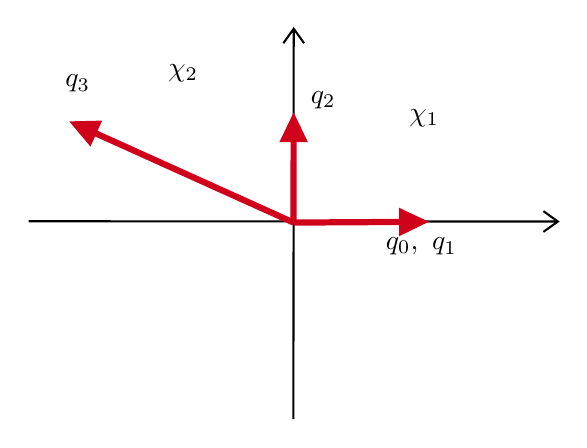
\begin{tikzpicture}[x=0.75pt,y=0.75pt,yscale=-1,xscale=1]
	%uncomment if require: \path (0,252); %set diagram left start at 0, and has height of 252
	
	%Shape: Axis 2D [id:dp521058933232561] 
	\draw [line width=0.75]  (220.97,123.04) -- (475.93,123.18)(348.65,30.28) -- (348.49,218.43) (468.93,118.17) -- (475.93,123.18) -- (468.92,128.17) (343.65,37.28) -- (348.65,30.28) -- (353.65,37.28)  ;
	%Straight Lines [id:da16836362624543133] 
	\draw [color={rgb, 255:red, 208; green, 2; blue, 27 }  ,draw opacity=1 ][line width=2.25]    (348.57,123.68) -- (348.61,75.61) ;
	\draw [shift={(348.62,70.61)}, rotate = 90.05] [fill={rgb, 255:red, 208; green, 2; blue, 27 }  ,fill opacity=1 ][line width=0.08]  [draw opacity=0] (14.29,-6.86) -- (0,0) -- (14.29,6.86) -- cycle    ;
	%Straight Lines [id:da8025190099366124] 
	\draw [color={rgb, 255:red, 208; green, 2; blue, 27 }  ,draw opacity=1 ][line width=2.25]    (348.57,123.68) -- (408.73,123.33) ;
	\draw [shift={(413.73,123.3)}, rotate = 179.67] [fill={rgb, 255:red, 208; green, 2; blue, 27 }  ,fill opacity=1 ][line width=0.08]  [draw opacity=0] (14.29,-6.86) -- (0,0) -- (14.29,6.86) -- cycle    ;
	%Straight Lines [id:da840019010653217] 
	\draw [color={rgb, 255:red, 208; green, 2; blue, 27 }  ,draw opacity=1 ][line width=2.25]    (348.57,123.68) -- (245.07,76.99) ;
	\draw [shift={(240.51,74.93)}, rotate = 24.28] [fill={rgb, 255:red, 208; green, 2; blue, 27 }  ,fill opacity=1 ][line width=0.08]  [draw opacity=0] (14.29,-6.86) -- (0,0) -- (14.29,6.86) -- cycle    ;
	
	% Text Node
	\draw (391.74,129.8) node [anchor=north west][inner sep=0.75pt]  [rotate=-0.04] [align=left] {$\displaystyle q_{0} ,\ q_{1}$};
	% Text Node
	\draw (355.61,59.24) node [anchor=north west][inner sep=0.75pt]  [rotate=-0.04] [align=left] {$\displaystyle q_{2}$};
	% Text Node
	\draw (237.33,51.28) node [anchor=north west][inner sep=0.75pt]  [rotate=-0.04] [align=left] {$\displaystyle q_{3}$};
	% Text Node
	\draw (403.06,67.91) node [anchor=north west][inner sep=0.75pt]  [rotate=-0.04] [align=left] {$\displaystyle \centerdot \chi _{1}$};
	% Text Node
	\draw (286.97,46.31) node [anchor=north west][inner sep=0.75pt]  [rotate=-0.04] [align=left] {$\displaystyle \centerdot \chi _{2}$};
	
	
\end{tikzpicture}
	
\end{centering}


Note that $\det V=(0,2)^T$
The characters define GIT quotients: 
\begin{itemize}
	\item  $X_{1}= \mathbb{C}^{4}//_{\chi_{1}}T^{2}= \mathbb{P}(\mathcal{O}_{\mathbb{P}^{1}}\oplus \mathcal{O}_{\mathbb{P}^{1}}(2)) = \mathbb{F}_2$
	\item  $X_{2}= \mathbb{C}^{4}//_{\chi_{2}}T^{2}= \mathbb{P}(1,1,2)$
\end{itemize}

Note that $\mathbb{F}_2$ is the minimal resolution of $\mathbb{P}(1,1,2)$, related by a blow up at its singular point.
\end{example}

Wall crossings can give us other standard birational transformations.

\begin{example}{Atiyah Flop}{Atiyah Flop}
Consider the action of $\mathbb{C}^{*}$ on $\mathbb{C}^3$ with weights $(1,1,-1)$. 
There are two quotients: $X_+$ corresponding to the chamber with the weights $(1,1)$, i.e. take the unstable locus to be $x=y= 0$, or $X_-$ corresponding to the chamber with -1, i.e. take unstable locus $z = 0$. With these stability conditions we have $$
X_{+}= \mathcal{O}(-1)_{\mathbb{P}^{1}} \qquad X_{-}= \mathbb{C}^2, $$ where the wall crossing from the $X_-$ to $X_+$ give the blow up at a point. 

Now suppose $\mathbb{C}^*$ now acts on $V = \mathbb{C}^4$  with coordinates $x_{1}, x_{2}, y_{1},y_{2}$, and weight matrix $Q = \begin{pmatrix}1&1&-1&-1\end{pmatrix}$. 
Defines two chambers in the secondary fan: $\chi_{+}>0$ and $\chi_{-}<0$, so we get unstable locus $x_{1}= x_{2}= 0$ and $y_{1}= y_{2}=0$. Hence $$
X_{+}\simeq \mathcal{O}(-1)_{\mathbb{P}^{1}}^{\oplus_{2}}\simeq X_-
$$This is an example of the Atiyah flop, related by a blow up and its flopping contraction. 
\end{example}

We say a variety is a minimal model if has nef canonical divisor. In the GIT picture, we say a GIT quotient is minimal if $-\det V$ lies in the closure of the chamber corresponding to the variety. 

\subsubsection{Wall Crossing Formula}

cf.~\cite*{Kite_2022,ballard2014variation} Let $V$ be a vector space of dimension $n$, and let $T$ be an algebraic torus.

Let $V$ be a vector space of dimension $n$, and let $T$ be an algebraic torus. Denote $\det V = \sum_i q_i$, where $q_i$ is the $i^\mathrm{th}$ column of the weight matrix $Q$. 

\begin{definition}{1-Parameter Subgroup}{1-PS}
    Given a reductive, linear algebraic group $G$, we call a one parameter subgroup of $G$ (the image of) an injective homomorphism $\lambda : \mathbb{G}_{m}\to G$. If $G$ acts on a space $V$, this induces an action of $\mathbb{G}_m$ on $V$ defined by $\lambda$, of which we denote the fixed locus $V^\lambda$. 
\end{definition}

Consider a toric GIT problem defined by the action of a group $T$ on a vector space $V$. Let $C_+$ and $C_-$ be adjacent chambers of the secondary fan in $L^{*}_\mathbb{R}$ separated by a wall $W$. Assume that $\det V$ is on the $C_{+}$ side of the adjoining wall $W$. The wall $W$ corresponds to an orthogonal (primitive) one-parameter subgroup $\lambda_{W}\in L$.

We can define a value $\kappa = (\det V)(\lambda_W)$. Let $\lambda_W$ be such that $\kappa \geq 0$, so is pointing to the $C_+$ 'side' of the wall. $\kappa$ is a combinatorial value which will (roughly) tell us which chamber admits the 'bigger' GIT quotients. 

Let $X_+$ (resp. $X_-$) be the GIT quotient $V // _{\theta_{+}}T$ (resp. $V // _{\theta_{-}}T$ ) corresponding to the chosen generic stability condition $\theta_{+}\in C_+$ (resp. $\theta_-$).  Recall from the previous section that GIT quotients are invariant across stability conditions in the interior of a given chamber. 

We can define a somewhat 'smaller' GIT problem associated to a subset $S \subset \{ 1,\dots,n \}$, or more specifically a subset $Q_S$ of the weights corresponding to the set $S$, which in our case are the $s_i$ columns of the weight matrix for $s_{i}\in S$. These weights generate a sublattice $L_{S}^{*}\subset L_\mathbb{R}^*$, determining what we call a Higgs GIT problem, defined by the exact sequence $$M_{S}\to \mathbb{Z}^{S}\xrightarrow{Q_{S}}L_{S}^{*}$$

From this we will now form a strictly lower dimensional variety $Z$ which give components in a SOD of $X_+$. First, we form a Higgs GIT problem, which defines the GIT quotient of the fixed locus $V^{\lambda_{W}}$ by the $T/\lambda_W$. Here, our subset $Q_S$  is the collection of weights which are orthogonal to $\lambda_W$, that is, the weights which lie in the space spanned by $W$. We can see that lattice $L_S^*$ is exactly the character lattice for the action of $T/\lambda_W$, since the the weights span the space orthogonal to $\lambda_W$. Moreover, the subspace of $V$ fixed by $\lambda_W$ corresponds to the lattice $\mathbb{Z}^S$ in the exact sequence. We choose a character $\theta_W$ in the chamber of $L_{S}^*$ define by the cone generated by $W$, to form the quotient $$Z = V^{\lambda_{W}} / /_{\theta_{W}} \left( T/ \lambda_{W}\right) . $$

Hence we get the theorem due to~\cite*{halpernleistner2014derived} and~\cite*{ballard2014variation}.

\begin{theorem}{Wall Crossing Formula}{wall crossing formula}
Consider GIT quotients $X_{+},X_{-}$  related by a wall crossing across the wall W as described above. 

If $\kappa > 0$, we have a semi-orthogonal decomposition given by $$D(X_{+}) = \left< D(X_{-}),D(Z) , \dots, D(Z)  \right>$$with $\kappa$ copies of $D(Z)$ appearing.

If $\kappa = 0$, the wall crossing induces a flop, and we have an equivalence of categories $$D(X_{+})\simeq D(X_-).$$
\end{theorem}

This theorem was proved in~\cite*{ballard2014variation} in much greater generality than used here, where such a decomposition holds for a smooth quasi-projective variety acted upon by a linear algebraic group, and a wall-crossing between two G-equivariant line bundles. However, to state the theorem in full generality requires more technical machinery than is necessary for the toric case for the purposes of our examples below. 

For ease of notation, we will denote the factor of $D(X)$ in a semi-orthogonal decomposition just as $X$. 

\begin{example}{}{}
    Recall Beilinson's exceptional collection~\cite*{Beilinson1978} which forms a SOD of $D(\mathbb{P}^n)$. Since $\mathbb{P}^n$ is a toric variety, we can realise it as the GIT quotient with respect to the usual action of $\mathbb{C}^*$ on $V = \mathbb{C}^{n+1}$. So the weights are $\begin{pmatrix}1 & 1 &\dots &1\end{pmatrix}$, with $\det V = n+1$. The wall crossing to $X_{-}=\emptyset$, retrieves the decomposition $\left< pt, \dots,pt \right>$ with $n+1$ copies of the derived category of a point, corresponding to the exceptional collection of line bundles on $\mathbb{P}^n$. 
\end{example}

\begin{example}{}{}
    Consider the action of $\mathbb{C}^{*}$ on $\mathbb{C}^3$ with weights $(1,1,-1)$. There are two stability conditions which can define toric GIT quotients, with $X_+$ corresponding to the chamber with the weights $(1,1)$, i.e. take the unstable locus to be $x=y= 0$, or $X_-$ corresponding to the chamber with -1, i.e. take unstable locus $z = 0$. With these stability conditions we have $$X_{+}= \mathcal{O}(-1)_{\mathbb{P}^{1}} \qquad X_{-}= \mathbb{C}^2, $$ Hence we get the have the decomposition $$D(\mathcal{O}(-1)_{\mathbb{P}^{1}})= \left< \mathbb{C}^{2}, pt \right> $$ which recovers Orlov's blow-up formula, as $X_+$ is the blow-up of $\mathbb{C}^2$ at a point.
\end{example}

\begin{example}{}{}
    Now consider the action of $\mathbb{C}^{*}$ on $\mathbb{C}^3$ with weights $(1,1,-2)$ corresponding to coordinates $x_{1},x_{2},y_1,y_2$ .  Since $\det V = 0$, any wall crossing will give us a flop. Indeed, we have stability conditions, giving quotients $$X_{+}= \mathcal{O}_{\mathbb{P}^{1}}(-2) \qquad X_{-}= [\mathbb{C}^{2}/ \mathbb{Z}_2]  $$where $[\mathbb{C}^2/\mathbb{Z}_2]$ is the orbifold with the action of $\mathbb{Z}_2$. The theorem thus gives us a derived equivalence $$D(\mathcal{O}_{\mathbb{P}^{1}}(-2))\simeq D([\mathbb{C}^{2}/\mathbb{Z}_{2}])$$
\end{example}


\subsubsection{Homological Mori Program}

The above theorem immediately yields a method for calculating a semi-orthogonal decomposition which is 'maximally refined', in that none of its components can be factored further through wall-crossings. This follows a similar algorithm to the MMP for toric GIT quotients. 

Starting with some fixed stability condition $\theta _1$ and its corresponding variety $X_1$, a wall crossing across the wall $W$ (away from $\det V$) gives the decomposition into $X_2$, the variety defined by the wall crossing, and $\kappa$ copies of the variety $Z_W$, the variety defined by the Higgs GIT problem for $W$. We can perform repeated wall crossings to decompose $X_2$ until a minimal model $X_{min}$ is reached. We will then be left with a factor of $X_{min}$ , and factors corresponding to the GIT problems $V^{\lambda_{W}} / / \lambda_{W}$ for each wall $W$ crossed, and can hence repeat the process of decomposition on each of the remaining non-minimal factors.

\begin{example}{Running the toric Mori program}{}
	ADD MORI PROGRAM EXAMPLE
\end{example}

We are interested in finding examples of nontrivial equivalences of derived categories induced by flops, which in the toric picture can be seen by considering the Calabi-Yau case.From this, it is clear that $\kappa = 0$ for all walls $W$ in the secondary fan, so any wall crossing induces a flop on the GIT quotients. Moreover, this gives us a way to see the nontrivial autoequivalences which come from these wall crossings. In particular, we will see that these autoequivalences have a nice interpretation as twists around spherical functors. 


\subsubsection{Relation to Mirror Symmetry}
cf


\subsection{Windows and Spherical functors}

First, we want to make some generalizations on the theory of spherical objects. Recall that a spherical object $\mathcal{E} \in D(X)$ satisfies the property that $$\mathrm{Hom}(\mathcal{E}, \mathcal{E}[i])= \begin{cases}
\mathbb{C} & i=0,\mathrm{dim}X  \\
0 & \text{otherwise}
\end{cases}$$
and the spherical twist of an object $\mathcal{F}$ around $\mathcal{E}$ is an autoequivalence defined as the cone $$T_\mathcal{E} = C(\mathrm{Hom}(\mathcal{E},\mathcal{F})\otimes \mathcal{E}\xrightarrow{ev} \mathcal{F})$$
We define spherical functors analogously.


\begin{definition}{}{}
	A functorial exact triangle is a 'triangle' of exact functors $F_{1}, F_{2}, F_{3} : \mathcal{C}\to \mathcal{D}$,    equipped with natural transformations $$
F_{1}(-)\to F_{2}(-)\to F_{3}(-)\to F_{1}(-)[1]
$$ such that for every object $\mathcal{F}\in \mathcal{C}$,   we get the exact triangle in $\mathcal{D}$ given by $$
F_{1}(\mathcal{F})\to F_{2}(\mathcal{F})\to F_{3}(\mathcal{F})\to F_{1}(\mathcal{F})[1]
$$
\end{definition}

Consider an adjoint pair of exact functors $L \dashv R$. Let $\eta : \mathrm{Id}_\mathcal{D}\to R\circ L$ be the unit and $\epsilon : L\circ R \to \mathrm{Id}_\mathcal{C}$ the counit. 

\begin{definition}{}{}
A functor between triangulated categories $F: \mathcal{A}\to \mathcal{B}$ is called spherical if it admits an adjunction $F^{*}\dashv F$ and  functorial exact triangles 
\begin{align}
F^{*}F \xrightarrow{\epsilon} \mathrm{Id}_\mathcal{A}&\to T \to F^{*}F [1] \\
C\to \mathrm{Id}_\mathcal{B}&\xrightarrow{\eta} F F^{*}\to C[1]
\end{align} such that $T$ and $C$ are equivalences. Then we call $T$ (resp. $C$) the spherical twist(resp. cotwist) along $F$. 
\end{definition}

Let $X_+$ and $X_-$ be two toric varieties related by a flop induced from a wall crossing in a Calabi-Yau GIT problem. In the formulation of the wall-crossing decomposition, we get a variety $Z$ from the wall $W$ which may appear in as a factor. $Z$ is the toric variety arising from the GIT problem induced by a character on the ray spanned by the wall. In ~\cite*{halpernleistner2016autoequivalences}, they show that we have countably infinitely many equivalences $\psi_{i}: D(X_{-})\xrightarrow{\sim} D(X_{+})$  such that the autoequivalence $\psi_{i+1}^{-1}\circ \psi_i$ of $D(X_{-})$ is a spherical twist around a spherical functor $$F : \mathcal{G}\to D(X_{-})$$ for a category $\mathcal{G}$ (to be defined later).

We examine this twist in more detail for the case of the standard flop (cf.~\cite*{donovan_window_2014}) before stating the more general theorem. 

Recall once more the action of $T = \mathbb{C}^*$ on $V = \mathbb{C}^4$  acting on coordinates $x_{1}, x_{2}, y_{1},y_{2}$ with weights $\begin{pmatrix}1&1&-1&-1\end{pmatrix}$ respectively. So $X_+$ and $X_-$ are both isomorphic to $\mathcal{O}(-1)_{\mathbb{P}^1}^{\oplus_{2}}$, related by a flop along the zero section $\mathbb{P}^1_{x_{1},x_{2}}$ or vice versa. Clearly their derived categories are equivalent. Since $X_+$ and $X_-$ are the quotients of $V$ minus an unstable locus ($x_{1}= x_{2}= 0$ or $y_{1}= y_{2}=0$)  by $T = C^{*}$, we can view them as sub-quotient stacks of the Artin quotient stack $\mathfrak{X}=[V/T]$. Thus we can consider the derived category of $T$-equivariant sheaves on $V$, which we denote $D(\mathfrak{X})$. We thus have the inclusions $$
i_{\pm}: X_{\pm}\to \mathcal{X}
$$
Note that $D(\mathfrak{X})$ contains the line bundles $\mathcal{O}(i)$ (corresponding to characters of $\mathbb{C}^*$).  Hence we define subcategories of $D(\mathfrak{X})$ by $$
 \mathcal{W}_{t}= \left< \mathcal{O}(t), \mathcal{O}(t+1) \right> 
$$ for any $t \in \mathbb{Z}$. We can restrict the pullback of the inclusions to get equivalences $$
i^{*_{\pm}}:\mathcal{W}_{t} \xrightarrow{\sim} D(X_{\pm})
$$
This equivalence can be verified by considering that $X_\pm$ is a quasi-projective variety, so we can make use of Beilinson's theorem stating that $\mathcal{O}(t), \mathcal{O}(t+1)$ is a strong, full, exceptional collection on $\mathbb{P}^1$, so the direct summands of the bundle $\mathcal{O}(t)\oplus \mathcal{O}(t+1)$ generate  $D(\mathcal{O}(-1)_{\mathbb{P}^{1}}^{\oplus {2}})$.  Hence we can define the equivalence and then autoequivalence $$
\psi_{t}:= i_{+}\circ i_{-}^{*}: D(X_{-})\to D(X_{+}) \qquad \Phi_{t}:= \psi_{t-1}^{-1}\psi_{t}: D(X_{-})\to D(X_{-})
$$
We call $\mathcal{W}_t$ a window subcategory, in that $D(X_{-})$is passing through a smaller intermediate than the whole of $D(\mathfrak{X})$. Moreover, the autoequivalence can be composed from passing through any two windows, i.e. $$
w_{l,t}:= \psi_{l}^{-1}\psi_t
$$
This is called the 'window shift'. 

\begin{remark}{}{}
	The method from this examples can be generalized to the action of $\mathbb{C}^*$ on $\mathbb{C}^k$ so long as the GIT problem is still Calabi-Yau. Assuming the sum of the positive weights is $d$ (so the sum of the negative weights is $-d$), window shift autoequivalences can be constructed with the subcategory $$\mathcal{W}_{t}= \left< \mathcal{O}(t),\dots, \mathcal{O}(t+d-1) \right> $$
\end{remark}


Consider the effect of $\Phi_t$ on our generators $\mathcal{O}(t)$ and $\mathcal{O}(t+1)$. Clearly $\psi_t$ sends both line bundles to themselves on $X_{+}$. Next we apply $\psi_{t-1}^{-1}$, but first both line bundles need to be resolved in such a way that they are written in terms of $\mathcal{O}(t-1)$ and $\mathcal{O}(t)$. We already have this for $\mathcal{O}(t)$. For $\mathcal{O}(t+1)$, the pullback of the Euler sequence on the zero section $\mathbb{P}^1$ gives the Koszul resolution $$
 0\to \mathcal{O}(2)\xrightarrow{\begin{pmatrix}x_2\\-x_{1}\end{pmatrix}}\mathcal{O}(1)^{\oplus 2}\xrightarrow{\begin{pmatrix}x_{1}&x_2\end{pmatrix}} \mathcal{O}
$$so $\mathcal{O}(t+1)$ is quasi-isomorphic to the complex $\left[ \mathcal{O}(t)^{\oplus{2}}\to \mathcal{O}(t-1) \right]$, and we have image of each generator under $\Phi_t$ . 
\begin{align*}
\mathcal{O}(t) &\mapsto \mathcal{O}(t)\\
\mathcal{\mathcal{O}(t+1)}&\mapsto\left[ \mathcal{O}(t)^{\oplus 2}\to \mathcal{O}(t-1) \right][-1] .
\end{align*}

We can see that computing the image of an arbitrary object in $\mathcal{E} \in D(X_-)$ under $\Phi_t$ requires us to resolve $\mathcal{E}$ in terms of the generators of the first window, then resolve $\psi_{t}(\mathcal{E})$ in terms of generators of the second. This becomes more difficult in the general case.  SEGAL-DONOVAN shows the existence of an endofunctor on the ambient quotient stack $\mathfrak{T}: D(\mathfrak{X})\to D(\mathfrak{X})$ which identifies objects from one window with another, called the Transfer Functor. To see it in action, let's consider the case of $t = 1$.

Since both $X_-$ and $X_+$ have exceptional locus $\mathbb{P}^1$, which can both be contracted to a point giving us the following maps $$
\left\{ pt \right\} \xleftarrow{\pi} \mathbb{P}^{1}\xrightarrow{j} X_{-}
$$
This can be generalised to maps from the substack identified with the quotient of $\mathbb{C}^{2}_{y_{1}, y_{2}} \oplus \{ 0 \}$ by $\mathbb{C}^*$, giving the correspondence $$
\{ pt \}\xleftarrow{\Pi}[\mathbb{C}^{2}/\mathbb{C}^*] \xrightarrow{J} \mathcal{X}
$$
The transfer functor is then defined as the twist around the functor $\mathfrak{R}:= \Pi_{*}J^{!}: D(X_{-})\to D(\{ pt \})$  with left adjoint $\mathfrak{L}:= J_{*}\Pi^{*}$, given by $$
\mathfrak{T}:= \mathrm{Cone}\left(\mathfrak{L}\circ \mathfrak{R} \to \mathrm{Id}_{D(\mathfrak{X})} \right) 
$$
This functor restricts to an autoequivalence $T: D(X_{-})\to D(X_-)$ which is similarly the twist for the adjunction $L\dashv R= \pi_{*}j^{!} : D(X_{-})\to D(\left\{ pt \right\})$. That is, $T$ fits into a functorial exact triangle $$
L\circ R \xrightarrow{\epsilon} \mathrm{Id}_{D(X_{-})} \to T\to L\circ R[1]
$$Where $T$ is the cone on the counit $\epsilon$. 


\begin{theorem}{}{}
	~\cite*{donovan_window_2014} $T$ is the same as $\Phi_1$. 
\end{theorem}

\begin{proof}
	
The proof of this statement relies on $\mathfrak{T}$ satisfying three key conditions. 

First, $\mathfrak{T}$ must send $\mathcal{W}_1$ to $\mathcal{W}_{0}$. This follows from that fact that the relative canonical sheaf $\omega_J$ of $J$ is $\mathcal{O}(-2)$ with relative dimension $-2$, so we have 
\begin{align}
\Pi_{*}J^{!}(\mathcal{O}(1)) &= \Pi_{*}\left(\omega_{J}\otimes  J^{*} \mathcal{O}(1)[-2] \right) \\
&= \Pi_{*}\left( \mathcal{O}(-2)\otimes  J^{*}\mathcal{O}(1)[-2] \right) \\
&= \Pi_{*}\mathcal{O}(-1)[-2] \\
&=0  
\end{align}

Hence $\mathfrak{L} \circ \mathfrak{R} (\mathcal{O}(1))=0$, and so the cone on $\epsilon$ is the identity. Hence $\mathfrak{T}(\mathcal{O}(1)) = \mathcal{O}(1)\in \mathcal{W_0}$.

For $\mathcal{O}(2)$, 
\begin{align}
\Pi_{*}J^{!}(\mathcal{O}(2)) &= \Pi_{*}\left(\omega_{J}\otimes  J^{*} \mathcal{O}(2)[-2] \right) \\
&= \Pi_{*}\left( \mathcal{O}(-2)\otimes  J^{*}\mathcal{O}(2)[-2] \right) \\
&= \Pi_{*}\mathcal{O}[-2] \\
&= \mathcal{O}_{pt}[-2]
\end{align}

Pulling back from the point and pushing forward onto $\mathfrak{X}$, we get the sheaf $\mathcal{O}_{\mathbb{C}^{2}}[-2]$. We want to take the cone on the natural transformation $$
\mathcal{O}_{\mathbb{C}^2}[-2]\xrightarrow{\epsilon} \mathcal{O}(2)
$$ The exact sequence $$
0 \to \mathcal{O}(2)\to \mathcal{O}(1) ^{\oplus 2} \to \mathcal{O} \to \mathcal{O}_{\mathbb{C}^{2}}\to 0
$$ shows us that $\mathcal{O}_{\mathbb{C}^2}[-2]$ is quasi-isomorphic to $\left[ \mathcal{O}(2)\to \mathcal{O}(1)^{\oplus{2}}\to \mathcal{O} \right][-2]$, to taking the cone over $\epsilon$ gives us $\left[ \mathcal{O}^{\oplus{2}}\to \mathcal{O} \right][-1] \in \mathcal{W}_0.$

Hence we have 
\begin{align}
\mathcal{O}(1) &\mapsto \mathcal{O}(1) \\
\mathcal{O}(2) &\mapsto \left[ \mathcal{O}(1)^{\oplus_{2}}\to \mathcal{O} \right][-2] 
\end{align}

Which gives us the diagram

\[\begin{tikzcd}
	{\mathcal{W}_1} && {\mathcal{W}_0} \\
	& {D(X_+ )} \\
	{D(X_- )} && {D(X_- )}
	\arrow["{\mathfrak T}", from=1-1, to=1-3]
	\arrow["{i_+^*}"', from=1-1, to=2-2]
	\arrow["{i_- ^*}"', from=1-1, to=3-1]
	\arrow["{i_+^*}", from=1-3, to=2-2]
	\arrow["{i_- ^*}", from=1-3, to=3-3]
	\arrow["{\psi_1}", from=3-1, to=2-2]
	\arrow["T", from=3-1, to=3-3]
	\arrow["{\psi_0}"', from=3-3, to=2-2]
\end{tikzcd}\]

Secondly, the upper triangle commutes because $\mathfrak{T}$ must act trivially outside $\mathbb{C}^{2}_{y_{1},y_{2}}\oplus \{ 0 \}$, i.e. $$
i^{*}_{+}\mathfrak{T} = i^{*}_{+}
$$This is a given from the definition, since objects on $X_+$ are in the kernel of the composition $\mathfrak{L}\circ\mathfrak{R}$, so $\mathfrak{T}$ acts as the identity. 

Thirdly,  $\mathfrak{T}$ must restrict to $T$, i.e. the rectangle commutes. This is due to generators $\mathcal{O}$ and $\mathcal{O}(-1)$ not having higher cohomology, so the derived pushforwards $\pi_{*}$ and $\Pi_{*}$ at least give the same thing on $\mathcal{W}_1$ , so $i_{-}^{*}\circ \mathfrak{T} = T\circ i_{-}^{*}$. 

From these, we can conclude that the lower triangle commutes, so $T = \Phi_1$. 
\end{proof}

To relate this back to the usual reference of spherical twist we can look at the functorial exact triangle object-wise, to see that for each object $\mathcal{E}\in D(X_-)$, $T_F$ is the cone $$
T_{F}(E) = \mathrm{Cone}\left( \mathrm{Hom}(\mathcal{O}_{\mathbb{P}^{1}},\mathcal{E}) \otimes  \mathcal{O}_{\mathbb{P}^{1}} \to \mathcal{E}\right) 
$$ 

\begin{remark}{}{}
	This is just one example of a much more general statement about window shifts, and flops in general. \cite*{donovan_window_2014} prove the theorem for Grassmannian flops, which includes the case of the standard flop we just saw. Indeed, for  vector spaces $V$ and $S$ of dimension $d$ and $r \leq d$ respectively, the associated quotient stack for the GIT problem is $$
	\left[ \mathrm{Hom} (S,V) \oplus \mathrm{Hom}(V,S)/\mathrm{GL}(S) \right] 
	$$where the standard flop is the case when $d = 2$, $r=1$.
	\end{remark}


:Other generalizations:




